\documentclass{article}
\usepackage[utf8]{inputenc}
\usepackage{datetime}
\usepackage{enumerate}
\usepackage{textcomp}
\usepackage{amsmath}
\usepackage{tikz}
\usetikzlibrary{arrows}
\usepackage{graphicx}
\usepackage{amssymb}
\graphicspath{ {./images/} }
   
\title{\bf \Large ASSIGNMENT 10}
\author{Xinhao Luo}
\date{\today}

\def\math#1{$#1$} 

\setlength{\textheight}{8.5in}
\setlength{\textwidth}{6.5in}
\setlength{\oddsidemargin}{0in}
\setlength{\evensidemargin}{0in}
\voffset0.0in

\begin{document}
\maketitle
\medskip

\section{Exercise 6.1}
\begin{enumerate}[a)]
    \item 
        \begin{itemize}
            \item \math{m = [1, 0]; n = [20, 0]}
            \begin{equation}
                CosSim(m, n) = \frac{mn}{||m||||n||} = \frac{20}{20 \times 1} = 1
            \end{equation}
            \begin{equation}
                d(m, n) = ||m - m|| = 20 - 1 = 19
            \end{equation}
            \item \math{m =[20, 0], n = [0, 20]}
             \begin{equation}
                CosSim(m, n) = \frac{mn}{||m||||n||} = 0
            \end{equation}
            \begin{equation}
                d(m, n) = ||m - m|| = 20\sqrt{2}
            \end{equation}
        \end{itemize}
    \item If the origin changes, the relative distance between two points will stay the same. However, the CosSim will be affected, so euclidean distance should be use in order to keep the same measurement.
\end{enumerate}

\section{Exercise 6.2}

\begin{itemize}
    \item [\math{\pi(x) \geq \frac{1}{2}}] \begin{equation}
        e(f(x)) = P[f(x) \neq y] = P[y = -1] = 1 - \pi(x) = min(\pi(x), 1 - \pi(x))
    \end{equation}
    \item [\math{\pi(x) < \frac{1}{2}}] \begin{equation}
        e(f(x)) = P[f(x) \neq y] = P[y = 1] = \pi(x) = min(\pi(x), 1 - \pi(x))
    \end{equation}
\end{itemize}

\begin{equation}
    \begin{split}
        e(h(x)) &= P[h(x)=1]P[y = -1|x] + P(h(x) = -1) P[y = 1|x] \\
        &= P[h(x)=1]\pi(x) + P(h(x) = -1)(1 - \pi(x)) \\
        & \geq P[h(x)=1] min(\pi(x), 1 - \pi(x)) + P(h(x) = -1) min(\pi(x), 1 - \pi(x)) \\
        e(h(x)) &\geq min(\pi(x), 1 - \pi(x)) = e(f(x)) \\
    \end{split}
\end{equation}

\section{Problem 6.1}

\begin{enumerate}[a)]
    \item 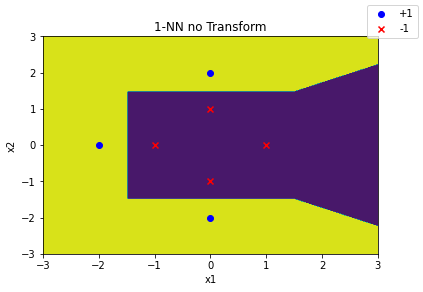
\includegraphics[]{1/1} \\ 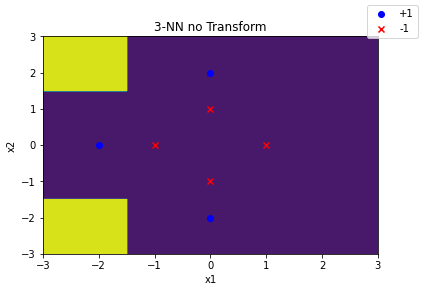
\includegraphics[]{1/2}
    \item 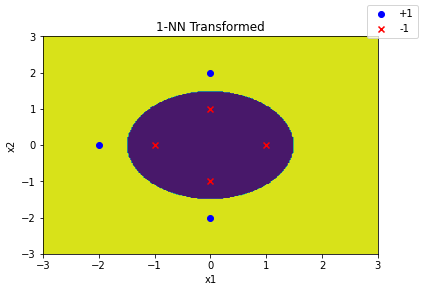
\includegraphics[]{1/3} \\ 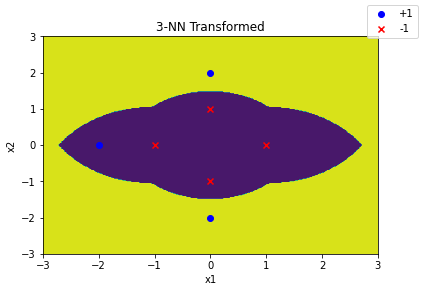
\includegraphics[]{1/4}
\end{enumerate}

\section{Problem 6.4}

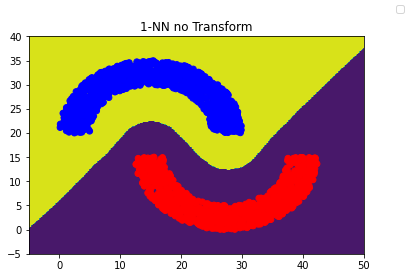
\includegraphics[]{2/1} \\
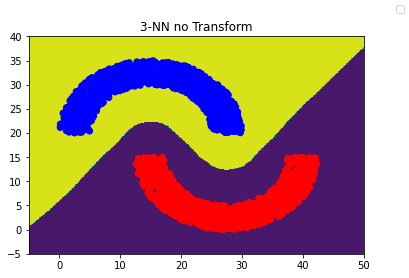
\includegraphics[]{2/2}

\section{Problem 6.16}

\begin{enumerate}[a)]
    \item 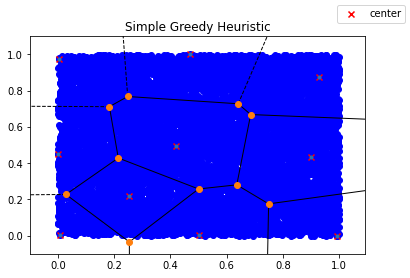
\includegraphics[]{3/1} \\ Brute Force: 220.972\\
    Branch and Bound: 21.145 \\
    Nearly 10x difference, branch and bound is much faster than brute force.
    \item 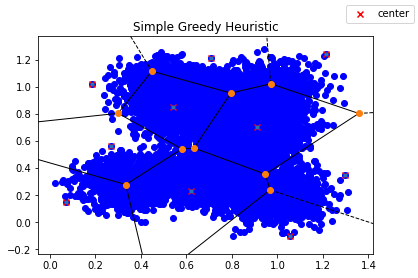
\includegraphics[]{3/2} \\ Brute Force: 252.183 \\
    Branch and Bound: 43.135
    \item In general, brute force is slower than branch and bound, but less effective in the b). It is possibly because branch and bound has exclude parts of the points from the distance calculation where brute force always calculate all points. However, b)'s points' distribution are more dense than a) so less points are excluded. 
    \item From result of a) and b), I would prefer branch and bound since in both cases \text{B\&B} shows better performance than brute force. In theory, there is an extra step for branch and bound: partition. If the data set is small, partition may lower the performance comparing with brute force; if the dataset is large and randomly distributed, it is hard to tell whether the partition will improve or worsen the performance. However, if the dataset is separated and well clustered, then branch and bound will always be better than brute force no matter the size of the data. On the other hand, if the data is clustered but their centers are close, branch and bound performance may be degraded to brute force or worse.
\end{enumerate}

\end{document}
